%%%%%%%%%%%%%%%%%%%%%%%%%%%%%%%%%%%%%%%%%%%%%%%%%%%%%%%%%%%
\section{Torque Control}
\label{sec:theory}
%%%%%%%%%%%%%%%%%%%%%%%%%%%%%%%%%%%%%%%%%%%%%%%%%%%%%%%%%%%
%\subsection{Controlling Torque}


The orientation of an object's major axis is important when a swarm is manipulating a non-symmetric object through narrow corridors. 
Orientation is controllable by applying torque to the object. 
To change the output torque $\tau$ in Eq.~\eqref{eq:torque}, we can choose the direction and magnitude of the force applied $F$, and the moment arm from the object's center of mass (COM) to the point of contact $r$.

\begin{equation}
\tau = F \times r\label{eq:torque}
\end{equation}
The swarm version of \eqref{eq:torque} is the summation of the forces contributed by individual robots.

\begin{align}
\tau_{total} &= \sum\limits_{i=1}^n \rho_i F_i \times (P_i - O )   \label{eq:swarmtorque}\\
F_{total} &= \sum\limits_{i=1}^n \rho_i F_i  \label{eq:swarmforce}
\end{align}

Here $F_i$ is the force that the $i$th robot applies.  If all robots are identical and the control input is uniform, the force is equivalent for every robot and $F_i = F_c$.
Not all robots are in contact with the object.  $\rho_i$ is an indicator variable: $\rho_i$ is 1 if the robot is in direct contact with the object or touching a chain of robots where at least one robot is in contact with the object. Otherwise $\rho_i = 0$.
The moment arm is the robot's position $P_i$ to the object's COM $O=[O_x,O_y]^{\top}$.

\section{Instantiation of torque from robot distribution}
Consider a swarm of robots with probability density $p(x)$. This section examines where to steer the mean of the probability distribution to maximize torque. We examine two problems. First, the torque applied to a rod of length 1 pivoted at 0 when $\theta = 0$ is:
\begin{equation}
\tau_{pivot} = \int_0^1 xp(x)\, dx
\end{equation}
Second, the torque applied to a free rod of length 2 from $[-1,0]$ to $[1,0]$, is:
\begin{equation}
\tau_{free} = \int_{-1}^1 xp(x)\, dx
\end{equation}
This section considers three canonical probability distributions: uniform, triangular, and normal. 

\begin{figure*}
\centering
\renewcommand{\figwid}{0.66\columnwidth}
\begin{overpic}[width =\figwid]{Uniform.pdf}%\put(1,55){a)}
\end{overpic}
\begin{overpic}[width =\figwid]{Triangular.pdf}
\end{overpic}
\begin{overpic}[width =\figwid]{Normal.pdf}
\end{overpic}
\vspace{-0.5em}
\caption{\label{fig:PDF} Three different distributions are examined in this work: uniform, triangular, and normal.
%\vspace{-2em}
}
\end{figure*}

\begin{figure*}
\centering
\renewcommand{\figwid}{0.66\columnwidth}
\begin{overpic}[width =\figwid]{TorqueUni.pdf}%\put(1,55){a)}
\end{overpic}
\begin{overpic}[width =\figwid]{TorqueTri.pdf}
\end{overpic}
\begin{overpic}[width =\figwid]{TorqueNormal.pdf}
\end{overpic}
\vspace{-0.5em}
\caption{\label{fig:torque} Torque with regard to mean position, $\mu$. Mean position is the pushing location.
%\vspace{-2em}
}
\end{figure*}
%uniform distribution
\begin{align}
p_u(x) &=  \left\{
\begin{array}{ll}
    \frac{1}{2\sqrt{3}\sigma}, &  \textrm{for   } \mu-\sqrt{3}\sigma \leq x \leq \mu+\sqrt{3}\sigma\\
     0, & \textrm{otherwise}\\
\end{array} 
\right.
\end{align}


%triangular distribution
\begin{align}
p_t(x) &=  \left\{
\begin{array}{ll}
    \frac{x-\mu + \sqrt{6} \sigma}{6\sigma^2}, &  \textrm{for   } \mu-\sqrt{6}\sigma \leq x \leq \mu\\
     \frac{-x+\mu + \sqrt{6} \sigma}{6\sigma^2}, &  \textrm{for   } \mu < x \leq \mu+ \sqrt{6}\sigma\\
     0, & \textrm{otherwise}\\
\end{array} 
\right.
\end{align}
%normal distribution
\begin{equation}
p_n(x) = \frac{1}{{\sigma \sqrt {2\pi } }}e^{{{ - \left( {x - \mu } \right)^2 } \mathord{\left/ {\vphantom {{ - \left( {x - \mu } \right)^2 } {2\sigma ^2 }}} \right. \kern-\nulldelimiterspace} {2\sigma ^2 }}}
\end{equation}

%defining torque uniform distribution
\begin{align}
l &= \max{0,\mu -\sqrt{3} \sigma}\\
u &= \min{1,\mu+\sqrt{3}\sigma}\\
\tau_u &= -\frac{l^2}{4\sqrt{3}\sigma}+ \frac{u^2}{4\sqrt{3}\sigma} \textrm{  for    }  u>l
\end{align}

%define torque for triangular:
\begin{align}
l_1 &= \max{0,\mu-\sqrt{6}\sigma}\\ \nonumber
l_2 &= \max{0,\mu}\\ \nonumber
u_1 &= \min{1,\mu}\\ \nonumber
u_2 &= \min{1,\mu+\sqrt{6}\sigma} \nonumber
\end{align}
\begin{align}
\tau_t &=  \left\{
\begin{array}{ll}
\frac{-2{l_1}^3+3{l_1}^2(\mu-\sqrt{6}\sigma)+{u_1}^2(2u_1 - 3\mu+3\sqrt{6}\sigma}{36\sigma^2}, &   \textrm{for     } u_1 > l_1\\
\frac{2{l_2}^3-3{l_2}^2(\mu+\sqrt{6}\sigma)+{u_2}^2(-2u_1 + 3\mu+3\sqrt{6}\sigma}{36\sigma^2}, &   \textrm{for     } u_2 > l_2\\
\end{array} 
\right.
\end{align}

%defining torque normal distribution
\begin{align} \nonumber
\tau_n &= \int_0^1\frac{1}{{\sigma \sqrt {2\pi } }}e^{{{ - \left( {x - \mu } \right)^2 } \mathord{\left/ {\vphantom {{ - \left( {x - \mu } \right)^2 } {2\sigma ^2 }}} \right. \kern-\nulldelimiterspace} {2\sigma ^2 }}} x \, dx\\ \nonumber
&= \frac{(-e^{-\frac{(-1+\mu)^2}{2\sigma^2}}+e^{-\frac{-\mu^2}{2\sigma^2}})\sigma}{\sqrt{2\pi}}\\ 
&+ \frac{1}{2}\mu(\erf(\frac{1-\mu}{\sqrt{2}\sigma})+\erf(\frac{\mu}{\sqrt{2}\sigma})) 
\end{align}



%taking derivative of torque
\begin{align} 
\frac{d\tau}{d\mu} &= -\frac{e^{-\frac{{-1+\mu}^2}{2\sigma^2}}}{\sqrt{2\pi}\sigma} + \frac{1}{2}(\erf(\frac{1-\mu}{\sqrt{2}\sigma})+\erf(\frac{\mu}{\sqrt{2}\sigma})) 
\end{align}


%%uniform torque
%\begin{align}
%\mu = \textrm{Max}[1-\sqrt{3}\sigma,\sqrt{3}\sigma]
%\end{align}




\section{Free object torque}
%torque uniform free
\begin{align}
l &= \max{-1,\mu -\sqrt{3} \sigma}\\
u &= \min{1,\mu+\sqrt{3}\sigma}\\
\tau_{uf} &= -\frac{l^2}{4\sqrt{3}\sigma}+ \frac{u^2}{4\sqrt{3}\sigma} \textrm{  for    }  u>l
\end{align}
%torque triangular free
\begin{align}
l_1 &= \max{-1,\mu-\sqrt{6}\sigma}\\ \nonumber
l_2 &= \max{-1,\mu}\\ \nonumber
u_1 &= \min{1,\mu}\\ \nonumber
u_2 &= \min{1,\mu+\sqrt{6}\sigma} \nonumber
\end{align}
\begin{align}
\tau_{tf} &=  \left\{
\begin{array}{ll}
\frac{-2{l_1}^3+3{l_1}^2(\mu-\sqrt{6}\sigma)+{u_1}^2(2u_1 - 3\mu+3\sqrt{6}\sigma}{36\sigma^2}, &   \textrm{for     } u_1 > l_1\\
\frac{2{l_2}^3-3{l_2}^2(\mu+\sqrt{6}\sigma)+{u_2}^2(-2u_1 + 3\mu+3\sqrt{6}\sigma}{36\sigma^2}, &   \textrm{for     } u_2 > l_2\\
\end{array} 
\right.
\end{align}

%torque normal free

\begin{align} \nonumber
\tau_{nf} &= \int_{-1}^1\frac{1}{{\sigma \sqrt {2\pi } }}e^{{{ - \left( {x - \mu } \right)^2 } \mathord{\left/ {\vphantom {{ - \left( {x - \mu } \right)^2 } {2\sigma ^2 }}} \right. \kern-\nulldelimiterspace} {2\sigma ^2 }}} x \, dx\\
 &= \frac{(-e^{-\frac{(-1+\mu)^2}{2\sigma^2}}+e^{-\frac{-(1+\mu)^2}{2\sigma^2}})\sigma}{\sqrt{2\pi}}\\
 &+ \frac{1}{2}\mu(\erf(\frac{1-\mu}{\sqrt{2}\sigma})+\erf(\frac{1+\mu}{\sqrt{2}\sigma})) 
\end{align}

%limits and equations

Consider robots are uniformly distributed. Finding the best place to guide the mean position:
% best place to push for uniform
\begin{align}
\left\{
\begin{array}{ll}
\mu = 1-\sqrt{3}\sigma &   \textrm{for     } \sigma > \frac{1}{2\sqrt{3}}\\
\mu = \sqrt{3}\sigma &   \textrm{otherwise}\\
\end{array} 
\right.
\end{align}
%best place to push for triangular:

%best place to push for normal distribution:
For triangular and normal distributions, the best place to push if $\sigma = 0$ is 1. The best place to push moves in the $x$ direction when $\sigma$ gets bigger. We used L'hopital rule and found third derivative of the torque to find the limit when standard deviation goes to infinity. It was because the first derivative had undefined numerator and denominator and we were not able to calculate it. The result is:

\begin{align}
\lim_{\sigma\to\infty} \frac{d^3x}{d\mu}(\tau_n)= -1+\frac{3\mu}{2}
\end{align}

which means the best position to push the rod moves left until it reaches $\mu = \frac{2}{3}$.

%pivoted comparisons:
\begin{figure*}
\centering
\renewcommand{\figwid}{\columnwidth}
\begin{overpic}[width =\figwid]{BestLocationPivot.pdf}%\put(1,55){a)}
\end{overpic}
\begin{overpic}[width =\figwid]{TorqueFreeBestPush.pdf}
\end{overpic}
\vspace{-0.5em}
\caption{\label{fig:bestLoc} Best location to push in two different situations: when the object is pivoted, and when the object is free.
%\vspace{-2em}
}
\end{figure*}

%\begin{figure}
%\begin{center}
%	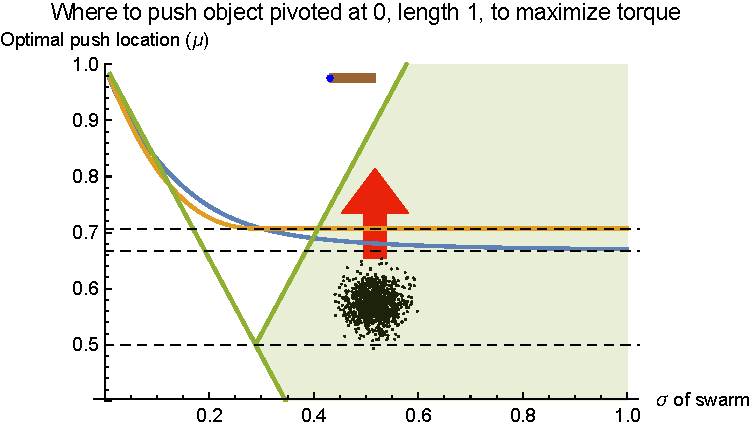
\includegraphics[width=0.8\columnwidth]{BestLocationPivot.pdf}
%\end{center}
%\vspace{-1em}
%\caption{\label{fig:besLocPiv}
%Comparison for three different distributions for the best location to push the object.
%}
%\vspace{0em}
%\end{figure}

\begin{figure*}
\centering
\renewcommand{\figwid}{\columnwidth}
\begin{overpic}[width =\figwid]{MaxTorquePivot.pdf}%\put(1,55){a)}
\end{overpic}
\begin{overpic}[width =\figwid]{TorqueFreeComparison.pdf}
\end{overpic}
\vspace{-0.5em}
\caption{\label{fig:maxTorque} Maximum torque possible in two situations: pivoted object and free object.
%\vspace{-2em}
}
\end{figure*}

%\begin{figure}
%\begin{center}
%	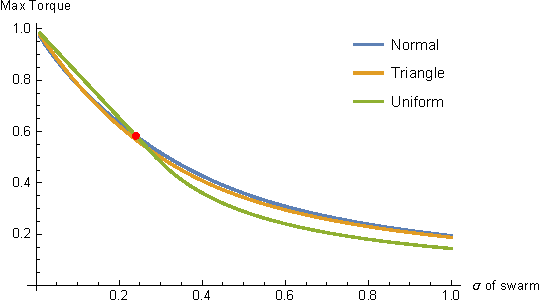
\includegraphics[width=0.8\columnwidth]{MaxTorquePivot.pdf}
%\end{center}
%%\vspace{0em}
%\caption{\label{fig:maxTorPiv}
%Comparison for three different distributions for the maximum torque possible.
%}
%\vspace{0em}
%\end{figure}
%
%%free comparisons
%
%\begin{figure}
%\begin{center}
%	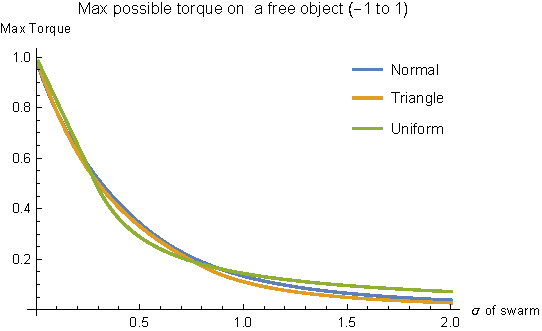
\includegraphics[width=0.8\columnwidth]{TorqueFreeComparison.pdf}
%\end{center}
%\vspace{-1em}
%\caption{\label{fig:maxTorqueFree}
%Comparison for three different distributions for the maximum torque possible.
%}
%\vspace{0em}
%\end{figure}


%\begin{figure}
%\begin{center}
%	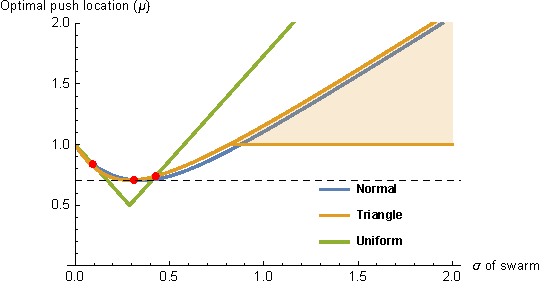
\includegraphics[width=0.8\columnwidth]{TorqueFreeBestPush.pdf}
%\end{center}
%%\vspace{0em}
%\caption{\label{fig:bestLocFree}
%Comparison for three different distributions for the best location to push the object.
%}
%\vspace{0em}
%\end{figure}


